\documentclass[./main.tex]{subfiles}

\begin{document}
\chapter{Implementation}\label{chap:impl}
\section{Data collection}\label{sec:implcollec}
The data is collected via MPU6050 gyroscope/accelerometer modules connected to
any microcontroller of choice (we have used both the NodeMCU and Arduino UNO
with success). These represent the edge nodes. We use one of Adafruit's
standard sensor libraries \cite{ada} (\mintinline{c}{Adafruit_MPU6050.h}) to interface
our edge nodes with the sensor.
\par

Each sensor's data is collected by listening for ``events'', that are passed to
a global \mintinline{c}{Adafruit_MPU6050} object.

\begin{code}
    \begin{minted}[bgcolor=codebg]{cpp}
    #include <Adafruit_MPU6050.h>

    Adafruit_MPU6050 mpu;
    bool reading_success;
    sensors_event_t accel_event, gyro_event, temp_event;
    \end{minted}
    \caption{Variable declaration}
    \label{code:ucvarinit}
\end{code}
\vspace{0.5cm}

The serial port also needs to be initialised along with the rest of the
objects. This is done in the \mintinline{c}{setup()} function. An
initialisation message is also printed to the serial port, to help with
synchronization later on.

\begin{code}
    \begin{minted}[bgcolor=codebg]{cpp}
    void setup()
    {
        Serial.begin(9600);
        mpu.begin();
        mpu.setAccelerometerRange(MPU6050_RANGE_16_G);
        mpu.setGyroRange(MPU6050_RANGE_2000_DEG);
        Serial.println("start");
    }
    \end{minted}
    \caption{Sensor setup}
    \label{code:ucsetup}
\end{code}
\vspace{0.5cm}

The sensor is then polled every 80 milliseconds for readings, and they are
printed as comma separated values to the serial port, for collection later use.
The units of the sensor readings that are sent to the serial port are:
\begin{itemize}
    \item Accelerometer: \unit{\metre\per\second}
    \item Gyroscope: \unit{\degree\per\second}
\end{itemize}

\begin{code}
    \begin{minted}[bgcolor=codebg]{cpp}
    void loop()
    {
        reading_success = mpu.getEvent(&accel_event, &gyro_event, &temp_event);
        if(reading_success) {
            Serial.print(accel_event.acceleration.x); Serial.print(",");
            Serial.print(accel_event.acceleration.y); Serial.print(",");
            Serial.print(accel_event.acceleration.z); Serial.print(",");
            Serial.print(gyro_event.gyro.roll * 180/M_PI); Serial.print(",");
            Serial.print(gyro_event.gyro.pitch * 180/M_PI); Serial.print(",");
            Serial.println(gyro_event.gyro.heading * 180/M_PI);
            delay(80);
        }
        else {
            Serial.println("Read unsuccessful");
        }
    }
    \end{minted}
    \caption{Main polling loop}
    \label{code:ucloop}
\end{code}
\vspace{0.5cm}

\section{Data storage}\label{sec:implstr}
Google Sheets is used as a database in this implementation. The data is read
from the serial port, and sent to a host node (see figure
\ref{fig:architecture}) that then updates Google Sheets via the REST API.

\subsection{Google Sheets API}
Google provides a RESTful API for Google Sheets via its cloud platform. Out of
the several REST resources available, we have used
\mintinline{c}{v4.spreadsheets.values} for updating the sheet. The sheet is
updated using the \mintinline{c}{batchUpdate} method \cite{gsheetapi}, which issues
\mintinline{c}{POST} requests, containing the range of cells, along with the
data to be updated.

\begin{itemize}
    \item HTTP Request:
        \begin{itemize}
            \item {\small \texttt{POST https://sheets.googleapis.com/v4/spreadsheets/\{spreadsheetId\}/values:batchUpdate}}
        \end{itemize}
\end{itemize}

\begin{table}[H]
\centering
\begin{tabularx}{\linewidth}{|X|X|}
    \hline
    \textbf{Field name} & \textbf{Field description} \\
    \hline
    \texttt{valueInputOption} & How the input data should be interpreted. \\
    \hline
    \texttt{data[]} & The new values to apply to the spreadsheet. \\
    \hline
\end{tabularx}
\caption{Used fields from request body \cite{gsheetapi}}
\label{fieldtable}
\end{table}

\begin{table}[H]
\centering
\begin{tabularx}{\linewidth}{|X|X|}
    \hline
    \textbf{Field name} & \textbf{Field description} \\
    \hline
    \texttt{spreadsheetId} &
    The spreadsheet the updates were applied to. \\
    \hline
    \texttt{totalUpdatedRows} &
    The total number of rows where at least one cell in the row was updated. \\
    \hline
    \texttt{totalUpdatedColumns} &
    The total number of columns where at least one cell in the column was
    updated. \\
    \hline
    \texttt{totalUpdatedCells} &
    The total number of cells updated. \\
    \hline
    \texttt{totalUpdatedSheets} &
    The total number of sheets where at least one cell in the sheet was
    updated. \\
    \hline
    \texttt{responses[]} &
    One \texttt{UpdateValuesResponse} per requested range, in the same order as the
    requests appeared. \\
    \hline
\end{tabularx}
\caption{Fields in response body \cite{gsheetapi}}
\label{fieldtable}
\end{table}

\begin{code}
    {\Smallfont \mintinline{sh}{POST https://sheets.googleapis.com/v4/spreadsheets/[SPREADSHEETID]/values:batchUpdate?key=[API_KEY] HTTP/1.1}}
    \begin{minted}{sh}
    Authorization: Bearer [ACCESS_TOKEN]
    Accept: application/json
    Content-Type: application/json

    {
        "value_input_option": "RAW",
        "data": [
            {
                "majorDimension": "ROWS",
                "range": "A2:H17",
                "values": [
                    [
                        "21-06-2021",
                        "18:05:45",
                        "-2.75",
                        "4.12",
                        "7.74",
                        "-16.59",
                        "-4.33",
                        "-34.70"
                    ],
                    ...
                    (There can be more values)
                ]
            }
        ],
    }
    \end{minted}
    \captionof{listing}{Example request}
    \label{code:reqex}
\end{code}
\vspace{0.5cm}

In listing \ref{code:reqex}, the range of cells to update is interpreted as-
\begin{code}
    \begin{table}[H]
        \centering
        \begin{tabular}{c}
        \texttt{<top-left-corner-cell>:<bottom-right-corner-cell>}
        \end{tabular}
    \end{table}
\end{code}
Since the \texttt{majorDimension} is \texttt{ROWS}, it will fill in as many
rows as there are values. The number of entries in the \texttt{values} section
must match the size of the buffer (which will be discussed in a later section),
or unexpected behaviour may occur.

\subsection{Python implementation}
Libraries used:
\begin{itemize}
    \item \texttt{pySerial}: For reading the serial port
    \item \texttt{os}: For using environment variables
    \item \texttt{datetime}: For creating timestamps
    \item \texttt{argparse}: For parsing command-line arguments
    \item Google API libraries
        \begin{itemize}
            \item \texttt{google-api-python-client}
            \item \texttt{google-auth-httplib2}
            \item \texttt{google-auth-oauthlib}
        \end{itemize}
\end{itemize}

\subsubsection{Setting up credentials}
\begin{code}
    \begin{minted}[bgcolor=codebg]{python}
    import os
    from google.oauth2 import service_account
    from googleapiclient.discovery import build
    SPREADSHEET_ID = # The sheet ID of the target spreadsheet
    SCOPES = ['https://www.googleapis.com/auth/spreadsheets']
    SERVICE_ACCOUNT_FILE = os.getenv("SERVICE_ACCOUNT_FILE")

    credentials = None
    credentials = service_account.Credentials.from_service_account_file(
            SERVICE_ACCOUNT_FILE,
            scopes=SCOPES
            )
    service = build('sheets', 'v4', credentials=credentials)
    \end{minted}
    \caption{Set up API authentication}
    \label{code:apiauth}
\end{code}
\vspace{0.5cm}

A Google Cloud account is necessary for this to work.  Credentials are set up
using a JSON file that is obtained when creating a \textit{service account} on
the Google Cloud console. It is supplied using environment variables for
security.

\subsubsection{Initialising the serial port}
\begin{code}
    \begin{minted}[bgcolor=codebg]{python}
    import serial

    port = # name of port
    serialPort = serial.Serial(port, baudrate=9600)
    serialPort.flushInput()
    \end{minted}
    \caption{Initialise serial port}
    \label{code:initser}
\end{code}
\vspace{0.5cm}

The serial port object is initialised with the name of the port, and the baud
rate. It is important that the baud rate of the microcontroller and the one
used here match. The port is also flushed to clear out any junk.

\subsubsection{Reading the serial data and crafting the HTTP payload}
\begin{code}
    \begin{minted}[linenos,bgcolor=codebg]{python}
    corner_top_left_row = 2
    bufsize = 16
    while(True):
        try:
            curr_range = "A" + str(corner_top_left_row)
            curr_range += ":H" + str(corner_top_left_row + bufsize - 1)

            buffer = []
    \end{minted}
    \caption{Buffer initialisation}
    \label{code:initbuf}
\end{code}
\vspace{0.5cm}

The readings are read in an infinite loop. At each pass, the range string is
created, and the buffer is (re-)initialised. Buffering is done to stay under
the rate limits imposed by Google on the API.

\begin{code}
    \begin{minted}[linenos,firstnumber=last,bgcolor=codebg]{python}
            # Buffer fixed sets of rows, and send one buffer at a time to stay
            # within GCP rate limit
            for i in range(0, bufsize):
                val = []

                val.extend(
                datetime.now().strftime("%d-%m-%Y,%H:%M:%S"
                ).split(','))

                ser_bytes = serialPort.readline()

                val.extend(
                ser_bytes[0:len(ser_bytes) - 2].decode('utf-8').strip().split(',')
                )

                buffer.append(val)
    \end{minted}
    \caption{Populate the buffer}
    \label{code:popbuf}
\end{code}
\vspace{0.5cm}

The buffer is filled with rows of data. It's size is determined by the value of
\texttt{bufsize}. The order of elements in each buffer entry is important and
must match the columns in the Google Sheet, otherwise this will lead to
mis-predictions. In our case, each element in the buffer is structured as
follows:
\begin{code}
    \begin{table}[H]
        \centering
        \begin{tabular}{c}
            \texttt{[date, time, Ax, Ay, Az, Gx, Gy, Gz]}
        \end{tabular}
    \end{table}
    \caption{Value list format}
    \label{code:vallist}
\end{code}
\vspace{0.5cm}

Here, anything with the prefix ``A'' is an accelerometer reading, along the
respective axes. Anything prefixed with ``G'' is a gyroscope reading, along the
respective axes.

\begin{code}
    \begin{minted}[linenos,firstnumber=last,bgcolor=codebg]{python}
            #  Send buffer once it is full, by calling the Sheets API
            #  Ref: https://developers.google.com/sheets/api/reference/rest
            batch_update_values_request_body = {
                'value_input_option': 'RAW',
                'data': [
                    {
                        "majorDimension": "ROWS",
                        "range": curr_range,
                        "values": buffer
                    }
                ]
            }

            request = service.spreadsheets().values().batchUpdate(
                    spreadsheetId=SPREADSHEET_ID,
                    body=batch_update_values_request_body
                    )
            response = request.execute()

            count += 1
            corner_top_left_row += bufsize
        except KeyboardInterrupt:
            print("")
            print("Summary:")
            print("Total requests: {}".format(count))
            break
        except Exception as e:
            print(e)
            break
    \end{minted}
    \caption{Read serial data and send POST request}
    \label{code:initser}
\end{code}
\vspace{0.5cm}

The request body is structured as shown in listing \ref{code:reqex}, and the
POST request is sent via the \mintinline{python}{request.execute()} call. The
range is updated and this process repeats. Any exceptions are caught and
handled as shown.

\section{Data visualisation and analysis}\label{sec:implvis}
The front-end for data visualisation is also implemented in Python. The
libraries used are:
\begin{itemize}
    \item \texttt{streamlit}: Main visualisation framework
    \item \texttt{time}: For timing
    \item \texttt{numpy}: For \texttt{numpy} arrays
    \item \texttt{os}: For using environment variables
    \item Google API libraries
        \begin{itemize}
            \item \texttt{gspread}
            \item \texttt{google-auth-oauthlib}
        \end{itemize}
\end{itemize}

\begin{code}
    \begin{minted}[bgcolor=codebg]{python}
    from google.oauth2 import service_account
    import gspread
    import time
    import os
    import numpy as np
    import streamlit as st

    SCOPES = [
            'https://www.googleapis.com/auth/spreadsheets',
            'https://www.googleapis.com/auth/drive.file',
            'https://www.googleapis.com/auth/drive'
            ]
    SERVICE_ACCOUNT_FILE = os.getenv("SERVICE_ACCOUNT_FILE")
    \end{minted}
    \caption{Initialisation}
    \label{code:clsinit}
\end{code}
\vspace{0.5cm}

Streamlit provides an incredibly simple yet elegant framework for visualisation
of data. The front-end is entirely powered by a web-app created with Streamlit.
The object-oriented model used here is as follows:

\begin{code}
    \begin{minted}[bgcolor=codebg]{python}
    class GetData:
        def __init__(self):
            self.scope = SCOPES
            self.creds = service_account.Credentials.from_service_account_file(
                    SERVICE_ACCOUNT_FILE,
                    scopes=self.scope)
            self.client = gspread.authorize(self.creds)
            self.sheet = self.client.open("sheet_name").sheet1
            self.chart = st.line_chart(np.array([[5.0]]))
    \end{minted}
    \caption{The \mintinline{python}{getData} class}
    \label{code:getdatacls}
\end{code}

\subsection{Class methods}
\subsubsection{\mintinline{python}{gettime_insecs()}}
This method returns the time in seconds between a start time \texttt{st} and
end time \texttt{en}, which are \texttt{time.localtime} instances.

\begin{code}
    \begin{minted}[bgcolor=codebg]{python}
    def gettime_insecs():
        self.start_hr = st[3]
        self.start_min = st[4]
        self.start_sec = st[5]
        self.end_hr = en[3]
        self.end_min = en[4]
        self.end_sec = en[5]
        startSumSec = (self.start_hr * 3600)
                        + (self.start_min * 60)
                        + self.start_sec
        endSumSec = (self.end_hr * 3600) + (self.end_min * 60) + self.end_sec
        return endSumSec - startSumSec
    \end{minted}
    \caption{The \mintinline{python}{gettime_insecs} method}
    \label{code:gettime_insecs}
\end{code}

\subsubsection{\mintinline{python}{good_posturetime()}}
This method returns a tuple containing the duration for which a good posture
was held, along with the row index of the reading that was taken into account.

\begin{code}
    \begin{minted}[bgcolor=codebg]{python}
    def good_posturetime(self, val, cursor, thresh=-15):
        started = time.localtime(time.time())
        st.success("Good Posture")
        while val >= thresh:
            val = self.sheet.cell(cursor, 7).value
            val = float(val)
            self.chart.add_rows(np.array([[val]]))
            cursor += 2
            print(cursor)
            time.sleep(1)
        ended = time.localtime(time.time())
        return self.gettime_insecs(started, ended), cursor
    \end{minted}
    \caption{The \mintinline{python}{good_posturetime} method}
    \label{code:good_posturetime}
\end{code}

\subsubsection{\mintinline{python}{bad_posturetime()}}
This method returns a tuple containing the duration for which a bad posture
was held, along with the row index of the reading that was taken into account.

\begin{code}
    \begin{minted}[bgcolor=codebg]{python}
    def bad_posturetime(self, val, cursor, thresh=15):
        started = time.localtime(time.time())
        st.error("Bad Posture")
        while val <= thresh:
            val = self.sheet.cell(cursor, 7).value
            val = float(val)
            self.chart.add_rows(np.array([[val]]))
            cursor += 2
            time.sleep(1)
            print(cursor)
        ended = time.localtime(time.time())
        return self.gettime_insecs(started, ended), cursor
    \end{minted}
    \caption{The \mintinline{python}{bad_posturetime} method}
    \label{code:bad_posturetime}
\end{code}

\subsubsection{\mintinline{python}{start_read()}}
This method actually plots the readings in real-time on the front-end.
Appropriate notifications are shown when posture changes, to notify users of
the same. A real-time plot of the \texttt{Gy} parameter (discussed in listing
\ref{code:vallist}) is also shown. A ``posture swing'' is detected as a swing in
\texttt{Gy} readings by more than $\pm$ \qty{15}{\degree\per\second}.

\begin{code}
    \begin{minted}[bgcolor=codebg]{python}
    def start_read(self, startingPoint=2, required_col=7):
        cursor = startingPoint
        while True:
            try:
                val = self.sheet.cell(cursor, required_col).value
                val = float(val)
                print(val)
                if val > 15:
                    gtime, cursor = self.good_posturetime(val=val, cursor=cursor)
                    print(val)
                    st.write("Good Posture time in seconds:", gtime)
                    print(f'goodPosture:{gtime}')
                elif val < -15:
                    btime, cursor= self.bad_posturetime(val=val, cursor=cursor)
                    st.write("Bad Posture time in seconds:", btime)
                    print(val)
                    print(f'BadPosture:{btime}')
                else:
                    cursor += 1
                    self.chart.add_rows(np.array([[float(val)]]))
            except:
                    pass
    \end{minted}
    \caption{The \mintinline{python}{start_read} method}
    \label{code:start_read}
\end{code}

\begin{figure}[H]
    \centering
    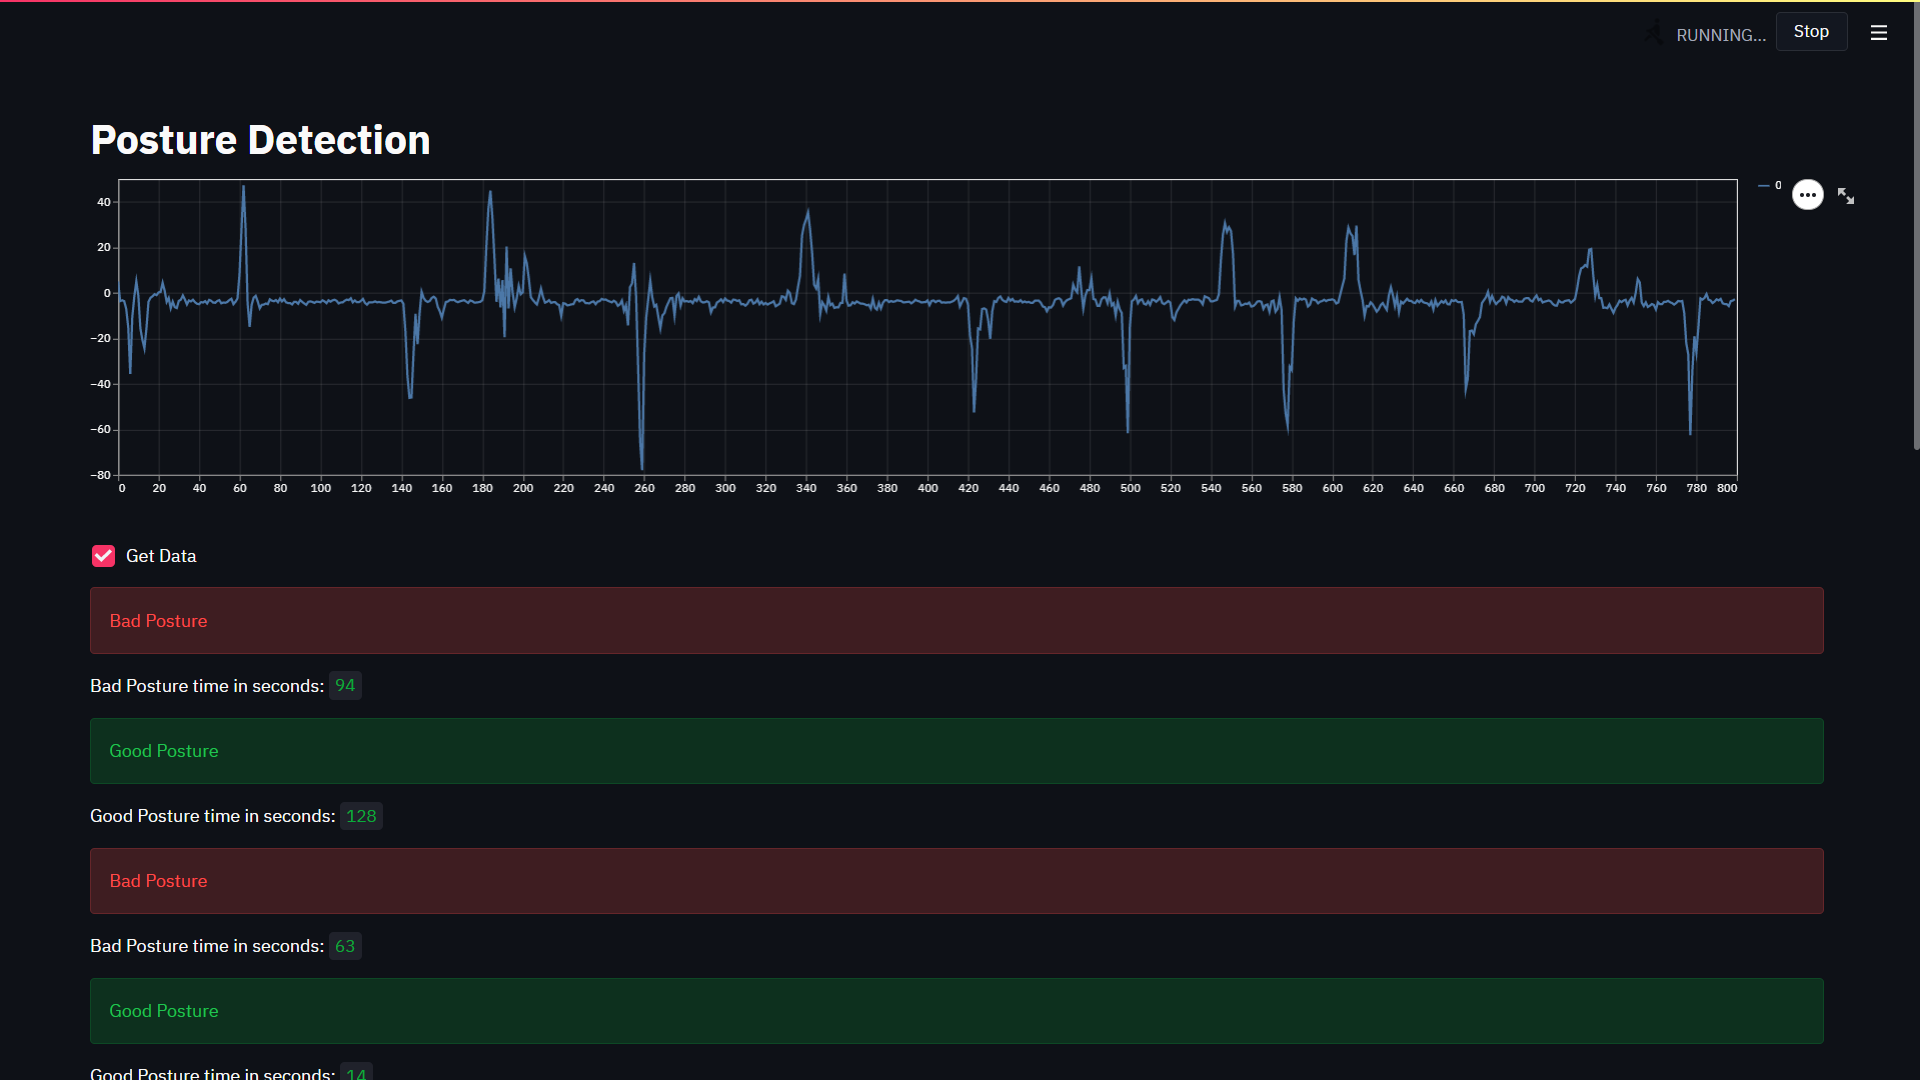
\includegraphics[scale=0.26]{webappss2.png}
    \caption{Web-app front-end}
    \label{fig:webapp}
\end{figure}

As shown in figure \ref{fig:webapp}, the graph on top shows a real-time
time-series representation of the \texttt{Gy} data. The notifications below the
graph correspond to the changes in posture.
\end{document}

